% pgfplots oracle fixture (hand-written): scopes inside `\foreach` bodies and
% brace groups of the axis body (behaviours V0, AB4, AC5): each iteration's
% plot takes the scope options; settings in a group or scope stay there.
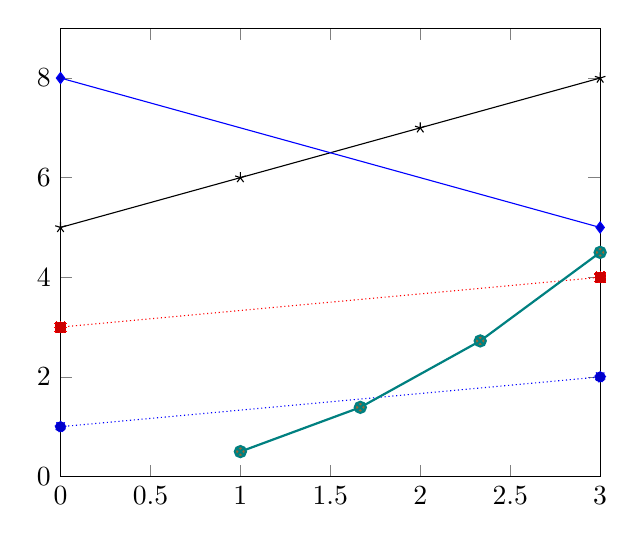
\begin{tikzpicture}
\begin{axis}[xmin=0, xmax=3, ymin=0, ymax=9, domain=0:3, samples=2]
\foreach \k in {1,3} {
  \begin{scope}[densely dotted]
    \addplot coordinates {(0,\k) (3,\k+1)};
  \end{scope}
}
{\pgfplotsset{samples=4}
  \begin{scope}[teal, thick]
    \pgfplotsset{domain=1:3}
    \addplot {x^2/2};
  \end{scope}
  \addplot {x+5};}
\addplot {8-x};
\end{axis}
\end{tikzpicture}
